\frame{\frametitle{Framework: Flask}
     	\begin{itemize}
		\item Microframework: 
		\begin{itemize}
			\item No tools or libraries required
			\item Easy to use for non-critical applications
		\end{itemize}
		\item Concepts:
		\begin{itemize}
			\item Instantiate Flask
			\item App routing to different endpoints
		\end{itemize}
		\item Can be used together with Plotly for interactive plot delivery
     	\end{itemize}
   }

\lstdefinestyle{mystyle}{
%    backgroundcolor=\color{backcolour},   
    commentstyle=\color{mLightGreen},
 %   keywordstyle=\textbf\color{mDarkTeal},
    %numberstyle=\tiny\color{codegray},
    stringstyle=\color{mLightBrown},
%    basicstyle=\ttfamily\footnotesize,
%    breakatwhitespace=false,         
%    breaklines=true,                 
%    captionpos=b,                    
%    keepspaces=true,                 
%    numbers=left,                    
%    numbersep=5pt,                  
%    showspaces=false,                
%    showstringspaces=false,
%    showtabs=false,                  
%    tabsize=2
}

\lstset{style=mystyle}

\frame{\frametitle{Import in WebApp (app.py)}
     	\lstinputlisting[language=Python, firstline = 1, lastline = 13]{App/app.py}
   }
   
 \frame{\frametitle{Create app}
     	\lstinputlisting[language=Python, firstline = 15, lastline = 16]{App/app.py}
   }

\begin{frame}[allowframebreaks]\frametitle{Preload data}
	Preloading of data at startup of the app speeds up the app significantly. For this we use the app route @app.before\_first\_request:
     	\lstinputlisting[language=Python, firstline = 18, lastline = 32]{App/app.py}
   \end{frame}
   
   \begin{frame}[allowframebreaks]\frametitle{Plot time series data}
   \begin{enumerate}
	\item  Define app route and and function:
     	\lstinputlisting[language=Python, firstline = 34, lastline = 35]{App/app.py}
	\item Open an error catching environment:
	\lstinputlisting[language=Python, firstline = 36, lastline = 36]{App/app.py}
	\item Declare the dataframe as global:
	\lstinputlisting[language=Python, firstline = 37, lastline = 37]{App/app.py}
	\item Generate the plot:
	\lstinputlisting[language=Python, firstline = 38, lastline = 47]{App/app.py}
	\item Transform the plot into a HTML div:
	\lstinputlisting[language=Python, firstline = 48, lastline = 51]{App/app.py}
	\item Render as HTML page, transferring the plotcode:
	\lstinputlisting[language=Python, firstline = 52, lastline = 52]{App/app.py}
	\newpage
	\item Catch the exception:
	\lstinputlisting[language=Python, firstline = 53, lastline = 55]{App/app.py}
	\end{enumerate}
	
   \end{frame}
   
   \frame{\frametitle{Start the app}
     	\lstinputlisting[language=Python, firstline = 106, lastline = 104]{App/app.py}
   }
   
    \begin{frame}[allowframebreaks]\frametitle{A geospatial plot on a different app route and in a different function}
     	\lstinputlisting[language=Python, firstline = 58, lastline = 104]{App/app.py}
   \end{frame}

\frame{\frametitle{Start the app}
\begin{columns}[t] 
     \begin{column}[T]{7cm} 
     	\begin{itemize}
		\item \texttt{cd} to App directory
		\item \texttt{python app.py}
		\item Apps works on localhost
     	\end{itemize}
     \end{column}
     	\begin{column}[T]{7cm} 
         	\begin{center}
            		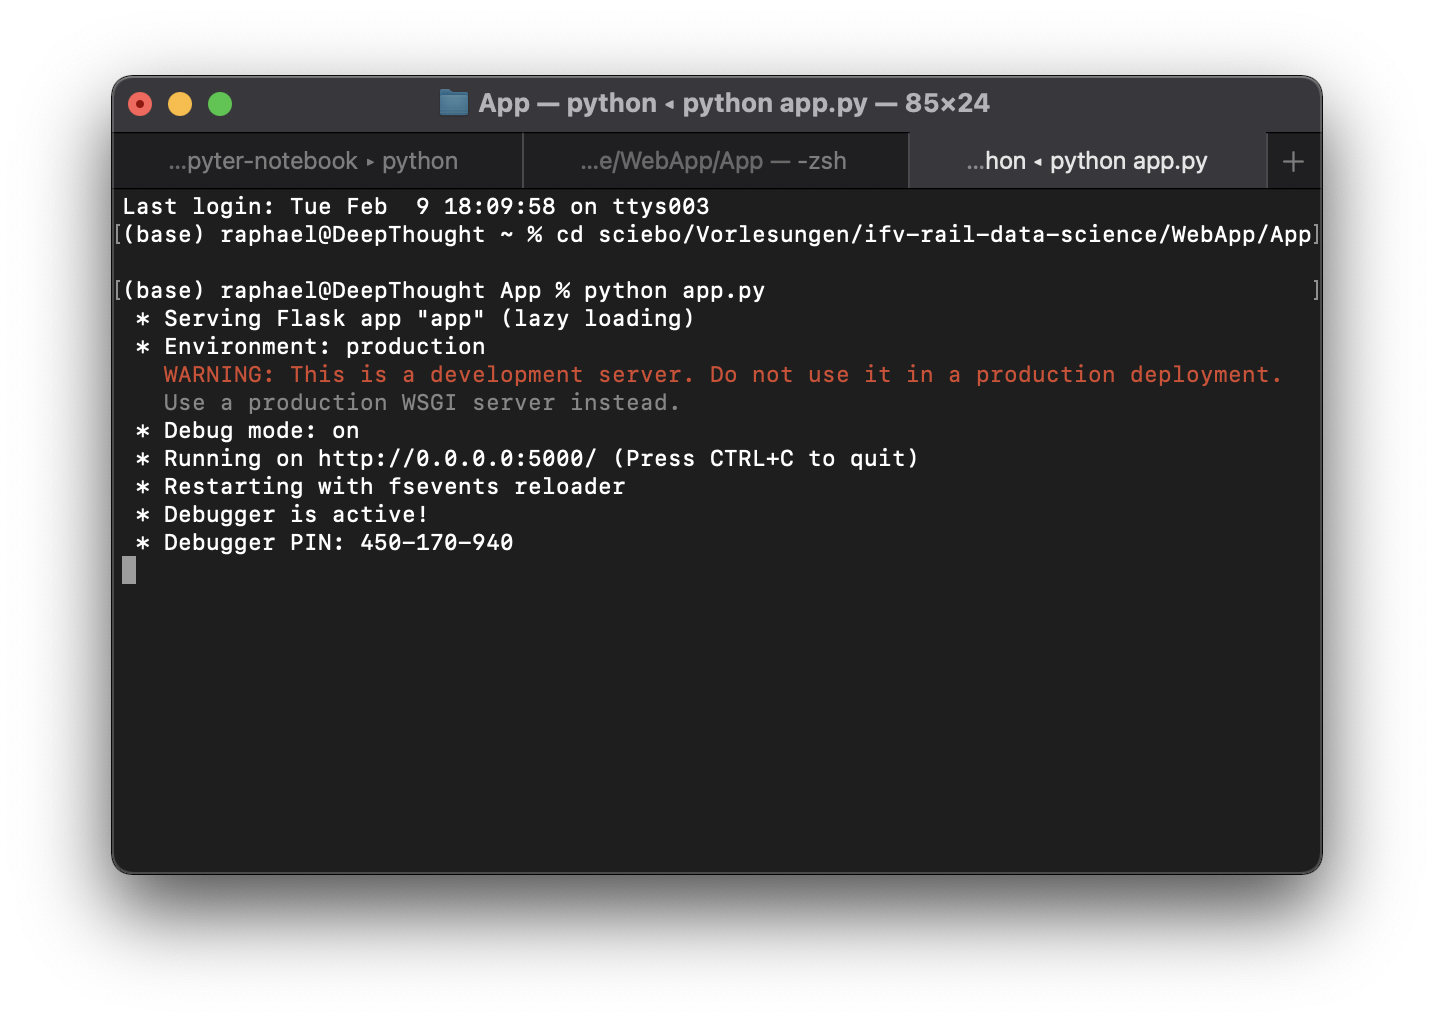
\includegraphics[width=0.95\textwidth]{startApp}\source{}
        		\end{center}
     \end{column}
 \end{columns}
}

\frame{\frametitle{Run the app}
\begin{columns}[t] 
     \begin{column}[T]{7cm} 
     	\begin{itemize}
		\item In a browser, visit \\
		\texttt{localhost:5000} \\
		and
		\item \texttt{localhost:5000/geo}
     	\end{itemize}
     \end{column}
     	\begin{column}[T]{7cm} 
         	\begin{center}
            		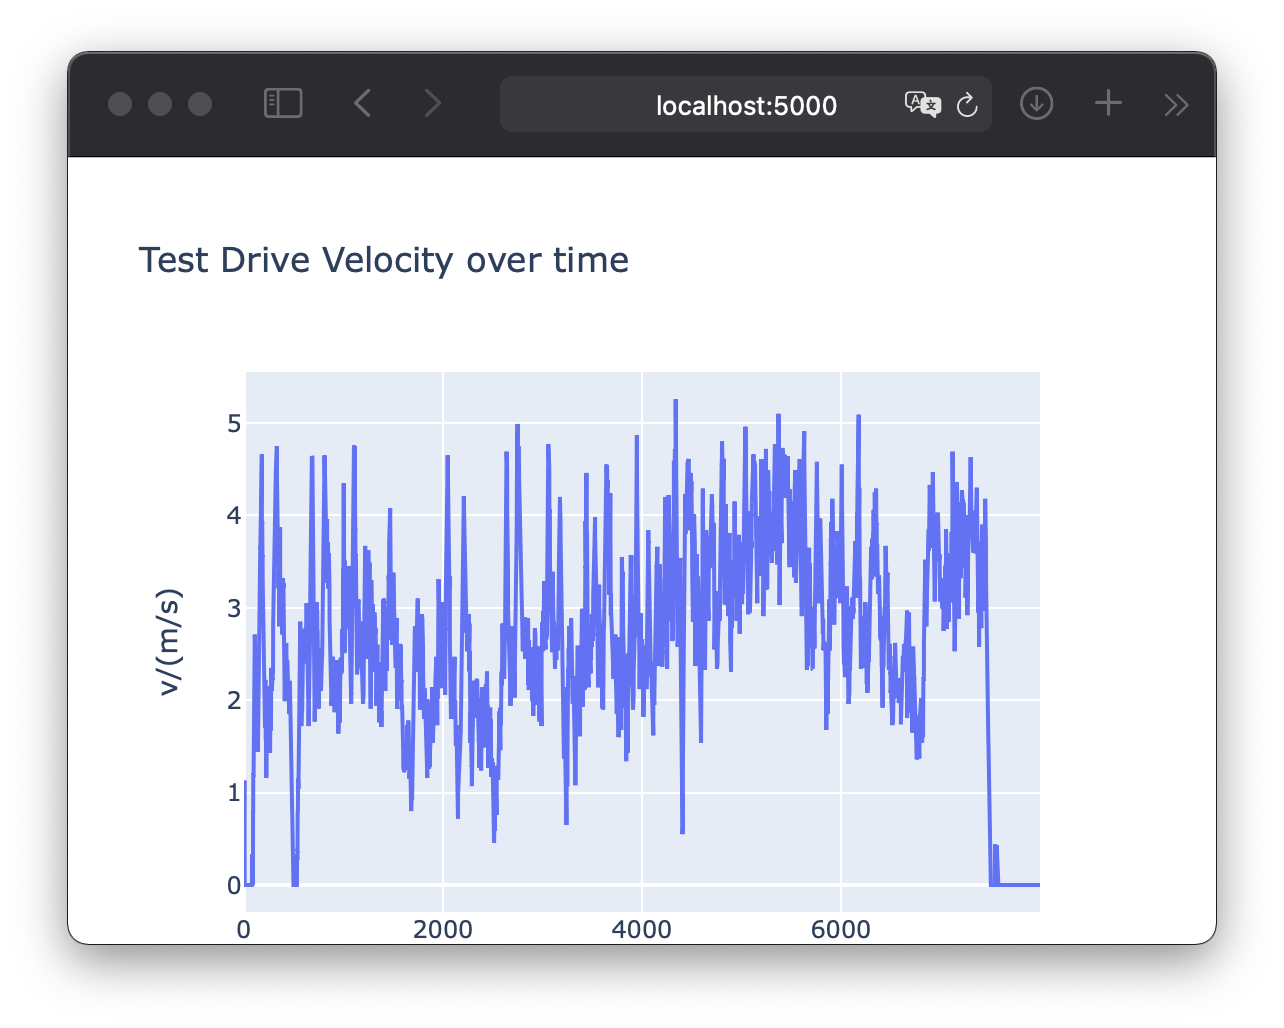
\includegraphics[width=0.55\textwidth]{App}\source{}
		\begin{flushright}
		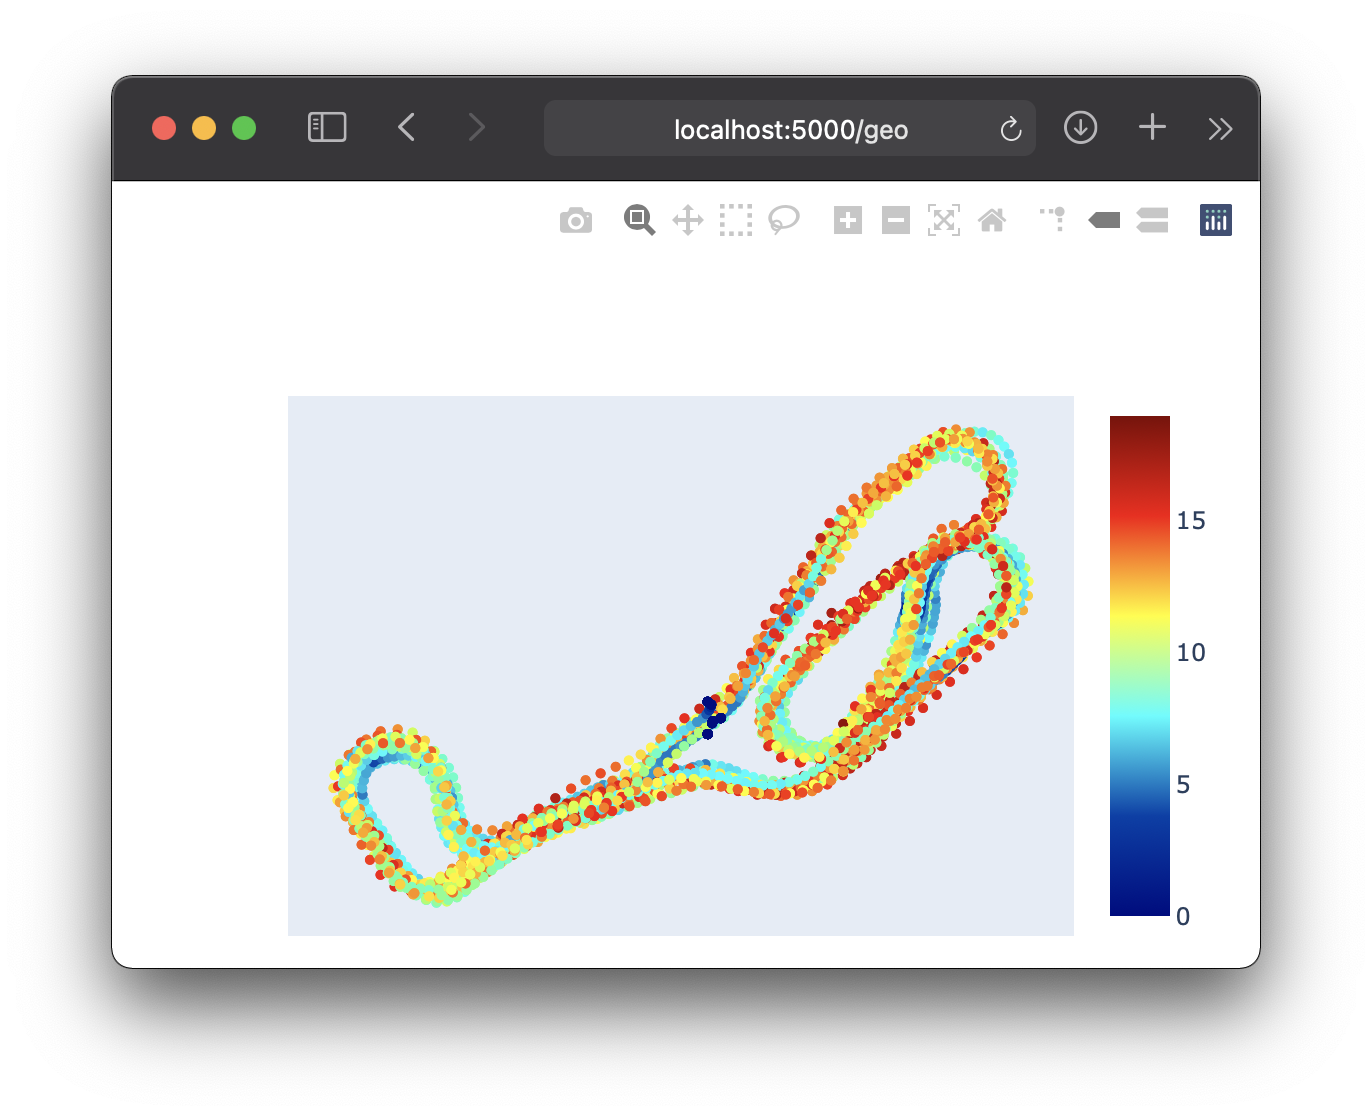
\includegraphics[width=0.55\textwidth]{Appgeo}\source{}
		\end{flushright}
        		\end{center}
     \end{column}
 \end{columns}
}

\frame{\frametitle{Exercise}
     	\begin{itemize}
		\item Extend the web app by adding another route \texttt{/hist} that delivers a plotly histogram
		\begin{itemize}
			\item To generate a histogram, use \texttt{data = go.histogram(x = df['v'])}
			\item The remainder of the plot code can stay mostly the same
		\end{itemize}
     	\end{itemize}
   }
